\documentclass[oneside,11pt,a4paper,italian]{article}

\PassOptionsToPackage{utf8}{inputenc}
 \usepackage{inputenc}				

\PassOptionsToPackage{T1}{fontenc} 
 \usepackage{fontenc}

\PassOptionsToPackage{italian}{babel}
 \usepackage{babel}

\PassOptionsToPackage{autostyle}{csquotes}
 \usepackage{csquotes}

\PassOptionsToPackage{italian}{varioref}
 \usepackage{varioref}

\PassOptionsToPackage{fleqn}{amsmath}
 \usepackage{amsmath}

\usepackage{siunitx,amssymb,braket,mhchem}

\usepackage[dvipsnames]{xcolor}%colors più fighi
\definecolor{halfgray}{gray}{0.55}

\usepackage{geometry,appendix}

\usepackage{tabularx} % better tables
	\setlength{\extrarowheight}{3pt} % increase table row height

\usepackage{caption}
\captionsetup{format=hang,font=small,labelfont={sf,bf}}

\usepackage{subfig,multirow,booktabs}

\usepackage{bm}

\usepackage{wrapfig}

\pdfcompresslevel=9
\pdfadjustspacing=1 
\PassOptionsToPackage{pdftex}{graphicx}
	\usepackage{graphicx}

\begin{document}
 \section{Comprensione bullet e variazione velocità diversi gas}
 L'obiettivo di questa analisi è spiegare la variazione di velocità variando la tensione di picco e il gas. Considero solo la velocità all'interno dell'ugello, dove il gas può essere considerato un gas ideale di elio o neon e stimo alcuni parametri del plasma, sotto diverse approssimazioni.
 
 Il campo elettrico $E$ è stimato come differenza di potenziale su una lunghezza tipica, \SI{30}{\milli\meter}, per avere un ordine di grandezza. La densità di corrente $j$ viene calcolata dalle intensità di corrente misurate quando il target è posto a \SI{30}{\milli\meter} dall'elettrodo (dove possibile), su una superficie circolare delle dimensioni misurate. La densità elettronica è $n_{e} = \frac{j}{e \mu E}$ con $e$ carica dell'elettrone e $\mu$ mobilità elettronica.
 
 La temperatura elettronica viene calcolata utilizzando \emph{BOLSIG+}, software risolutore dell'equazione di Boltzmann che considera le reazioni specifiche in un gas di elio o neon. Il software restituisce energia media e parametri di trasporto (mobilità, diffusione) al variare del campo elettrico ridotto $E/N$, dove $N$ è la densità dei neutri, pari a \SI{2.69e+25}{\meter^{-3}} per un gas ideale a pressione atmosferica. I parametri di mobilità elettronica restituiti da questo calcolo sono confrontabili con quelli trovabili in letteratura (Gas discharge physics, Raizer et al. ; The mobility of He+ ions in helium gas, Dickinson et al. ; Mobility and diffusion of atomic helium and neon ions in their parent gases, Skullerud et al.), dove si trovano anche cammino libero medio e mobilità per gli ioni, in tabella \ref{tab:pargas}.
 
 \begin{table}
  \centering
  \begin{tabular}{cccc}
  \toprule
  Gas    &$\mu_{e}$ [\si{\meter^2/\volt\second}]   &$\mu_{i}$ [\si{\meter^2/\volt\second}]   &$\lambda_{\text{MFP}}$ [\si{\meter}]\\
  \midrule
  He    &\num{0.114}    &\num{1.05e-3}  &\num{0.6e-3}\\
  Ne    &\num{0.198}    &\num{0.41e-3}  &\num{1.2e-3}\\
  \bottomrule
  \end{tabular}
  \caption{Parametri tipici di un plasma composto da elio o neon.}
  \label{tab:pargas}
 \end{table}

 
 Ho provato ad indagare principalmente due ipotesi:
 \begin{itemize}
  \item se il bullet visto fosse dovuto alla propagazione di onde di ionizzazione dentro il plasma, quindi se le velocità fossero compatibili con $c_{s,i} = \sqrt{\frac{\gamma Z k_{B} T_{e}}{m_{i}}}$
  \item se il bullet fosse il moto effettivo di ioni o elettroni, con velocità termiche $v_{th} = \sqrt{\frac{2 k_{B} T_{e}}{m}}$ o dovute al campo elettrico $v_{d} = \mu E$
 \end{itemize} 
 è importante notare che in realtà il plasma non credo soddisfi le condizioni di equilibrio necessarie alla definizione di temperatura elettronica, velocità termica e velocità delle onde, facendo questi calcoli sto ipotizzando che localmente sia tutto all'equilibrio.
 In tabella \ref{tab:vel} tutti i parametri stimati.
 
 \begin{table}
  \centering
  \begin{tabular}{cccccccc}
  \toprule
   &$V_p$ [kV]   &E [kV/m]   &$T_e$ [eV] &$c_{s}$ [km/s] &$v_{\text{th,e}}$ [km/s] &$v_{\text{d,e}}$ [km/s]    &$v_{\text{d,i}}$ [km/s]\\
  \midrule
   \multirow{3}*{He}    &5.7    &190    &4.5    &13.42  &14.73  &21.66  &0.20\\
                        &6.6    &220    &5.0    &14.15  &15.53  &25.08  &0.23\\
                        &7.3    &243    &5.5    &14.84  &16.29  &27.74  &0.26\\
  \midrule
  \multirow{3}*{Ne}     &4.8    &160    &6.8    &7.30  &8.06  &31.68  &0.066\\
                        &5.3    &177    &7.0    &7.41  &8.18  &34.99  &0.072\\
                        &6.1    &203    &7.2    &7.51  &8.30  &40.65  &0.083\\
  \bottomrule
  \end{tabular}
 \caption{Parametri stimati nei diversi setup.}
 \label{tab:vel}
 \end{table}

Qualsiasi fenomeno di spostamento degli ioni può essere scartato, considerando i valori di mobilità ionica e la temperatura del gas, le velocità di deriva e termiche per gli ioni sono al di sotto dei km/s.

Le velocità delle onde sono dello stesso ordine di grandezza di quelle viste per l'elio, ma troppo basse per il neon, e si ha un incongruenza con l'esperimento: dalle misure osserviamo velocità maggiori per il neon rispetto l'elio, mentre la velocità delle onde, essendo inversamente proporzionale alle masse, è minore per il neon.

Le velocità di deriva elettroniche sono dell'ordine di grandezza cercato e rispecchiano l'andamento dei dati: aumentando il campo elettrico crescono più velocemente per il neon rispetto l'elio. La costante di proporzionalità tra campo elettrico e velocità è proprio la mobilità elettronica, ma non avendo una misura diretta del campo elettrico non si può stimare direttamente questo parametro dalle misure. Andando a paragonare gli andamenti per elio e neon, come in figura \ref{fig:andmob}, troviamo che il rapporto tra le pendenze delle rette è $p_{\text{Ne}}/p_{\text{He}} = \num{1.60}$, mentre il rapporto tra le mobilità $\mu_{\text{Ne}}/\mu_{\text{He}} = \num{1.74}$, valori paragonabili. Interessante notare che se effettivamente la velocità è associabile ad un drift elettronico, vuol dire che il campo elettrico visto è dell'ordine di \SI{450}{\volt/\meter}, valore plausibile. 
\begin{figure}
 \centering
 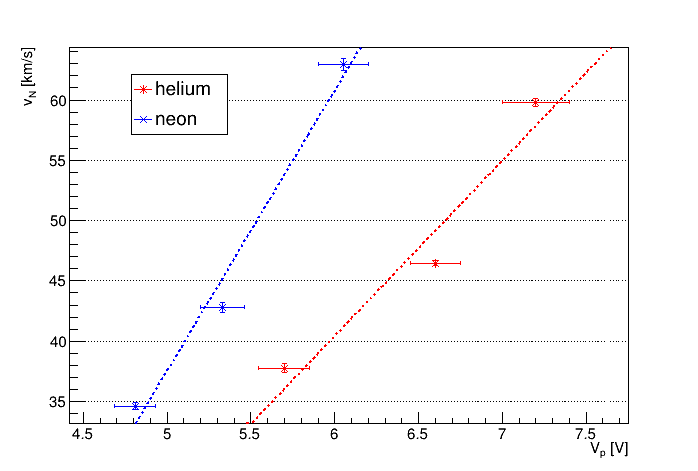
\includegraphics[width=0.52\textwidth]{../Images/Shape/hene_vN.png}
 \caption{Plot of bullet's velocity inside the nozzle increasing voltage, for helium and neon.}
 \label{fig:andmob}
\end{figure}


Se possiamo associare il moto del bullet al moto degli elettroni dentro il plasma, anche il cammino libero medio presentato in tabella \ref{tab:pargas} può essere associato alla dimensione del bullet ed il valore maggiore per il neon rispetto l'elio corrisponde all'effettiva misura di bullet più spessi per il plasma di neon.


\section{Diversi flussi numeri di Reynolds}
Ho calcolato il numero di Reynolds per i diversi flussi provati (formule e valori tipici in ``Influence of the gas-flow Reynolds numberon a plasma column in a glass tube'', Jin et al.), in tabella \ref{tab:rey} i risultati, trovando sempre valori inferiori ai valori di transizione da flusso laminare a turbolento ($\sim 2000$).

\begin{table}
  \centering
  \begin{tabular}{cccc}
  \toprule
  Q [L/min]   &$v_{N}$ [km/s]   &Re  &$x_{\text{air}}$ [\si{\milli\meter}]\\
  \midrule
  1    &\num{48.46}    &\num{36.88}  &\num{78.78}\\
  2    &\num{40.09}    &\num{73.77}  &\num{80.55}\\
  3    &\num{33.74}    &\num{110.65}  &\num{81.75}\\
  4    &\num{17.01}    &\num{147.54}  &\num{81.28}\\
  \bottomrule
  \end{tabular}
  \caption{Numeri di reynolds per diversi flussi di elio.}
  \label{tab:rey}
\end{table}


Osservando uno zoom sulle velocità dei bullet mentre escono dall'ugello, figura \ref{fig:zoom}, ipotizzerei che la velocità inferiore in uscita è data dal diverso punto di contatto tra aria e flusso di elio. Durante il moto dentro l'ugello il bullet e acquista velocità quando incontra l'aria esterna. Per flussi maggiori si ha il contatto tra elio e aria più tardi, in posizione più esterna, permettendo al bullet di rallentare prima notevolmente prima di venire espulso dall'ugello.
\begin{figure}
 \centering
 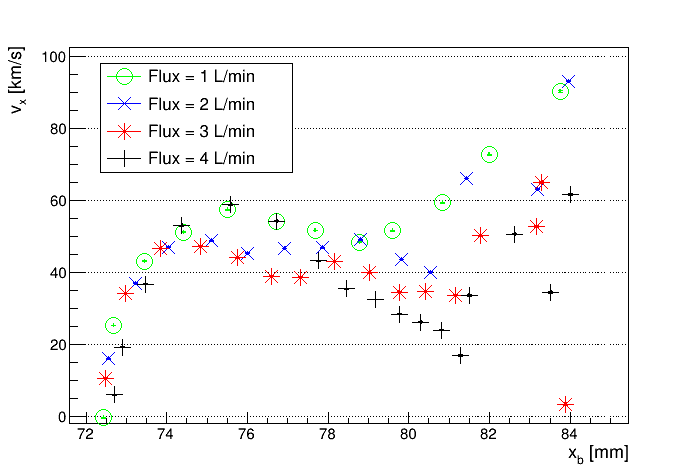
\includegraphics[width=0.52\textwidth]{../Images/Shape/vnoz_flux_zoom.png}
 \caption{Zoom sulle velocità dei bullet in uscita dall'ugello per i vari flussi.}
 \label{fig:zoom}
\end{figure}


\section{Intensità righe spettro}
Intensità totali e delle varie righe al variare della posizione \ref{fig:pos} e del flusso di gas (azoto o argon) \ref{fig:flux}.

\begin{figure}
 \centering
 \subfloat[Luminosità totale.]{
    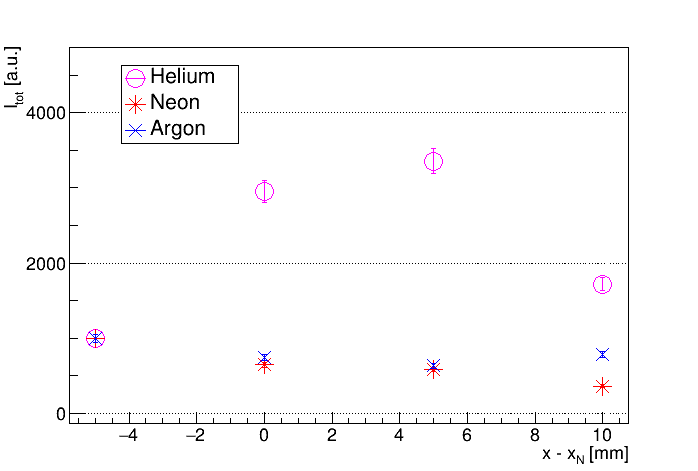
\includegraphics[width=0.45\textwidth]{../Images/Spectroscopy/Itot_pos.png}
 }
 \subfloat[Intensità delle righe NO.]{
    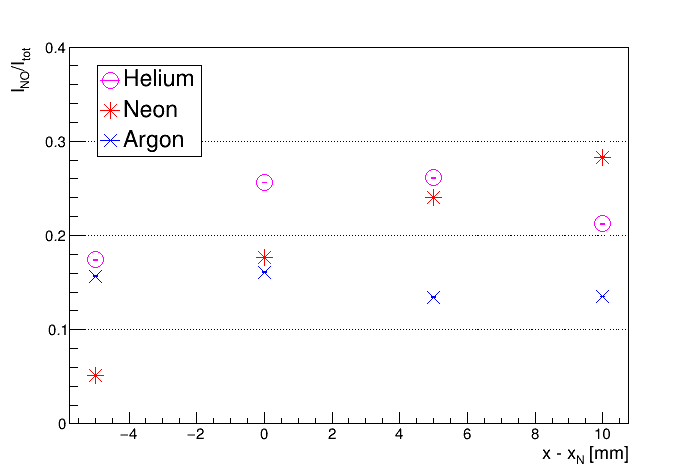
\includegraphics[width=0.45\textwidth]{../Images/Spectroscopy/Irel_NO_pos.png}
 }
 
 \subfloat[Intensità delle righe N2.]{
    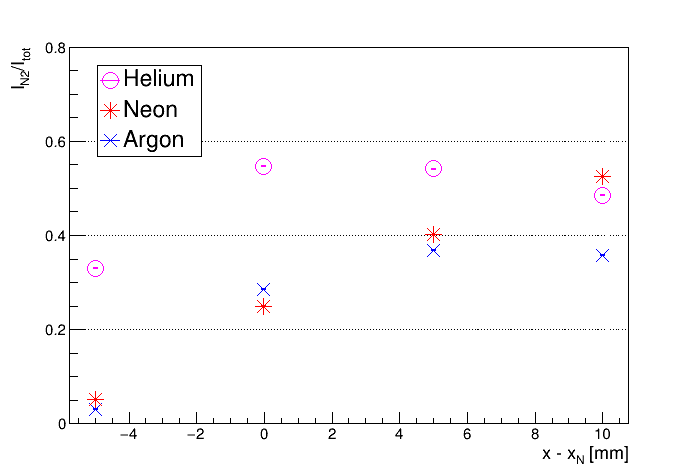
\includegraphics[width=0.45\textwidth]{../Images/Spectroscopy/Irel_N2_pos.png}
 }
 \subfloat[Intensità delle righe del gas utilizzato.]{
    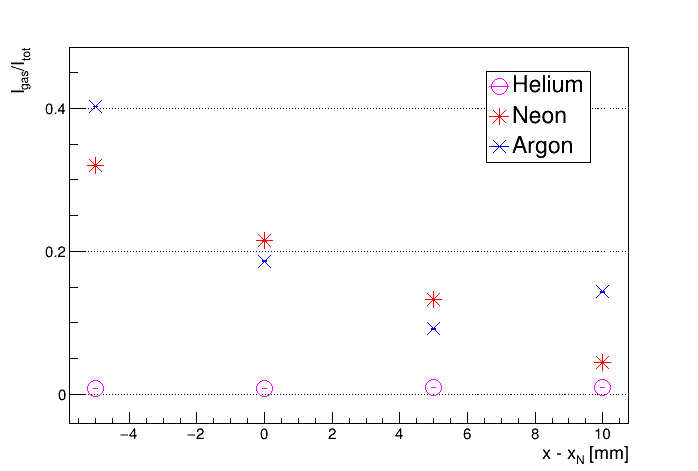
\includegraphics[width=0.45\textwidth]{../Images/Spectroscopy/Irel_gas_pos.png}
 }
 
 \caption{Intensità delle righe nello spettro al variare della posizione, $0$ della posizione sulla fine dell'ugello, target metallico in posizione $\SI{10}{\milli\meter}$. La luminosità totale è normalizzata arbitrariamente per i diversi gas, non sono paragonabili i valori per i diversi gas, se ne vuole solo indicare l'andamento.}
 \label{fig:pos}
\end{figure}

\begin{figure}
 \centering
 \subfloat[Luminosità totale.]{
    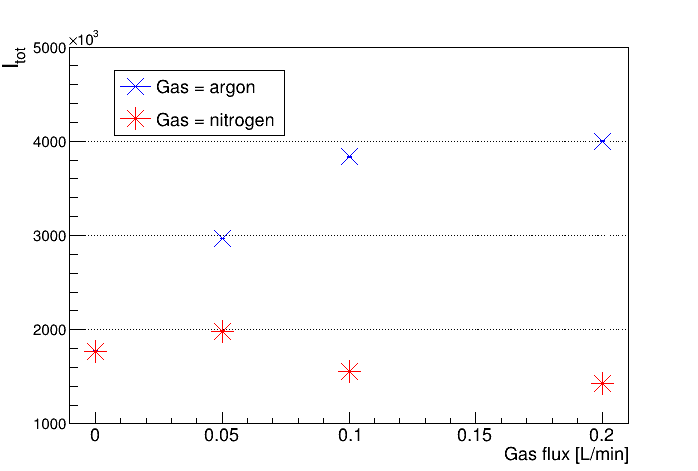
\includegraphics[width=0.45\textwidth]{../Images/Spectroscopy/Itot_flux.png}
 }
 \subfloat[Intensità delle righe NO.]{
    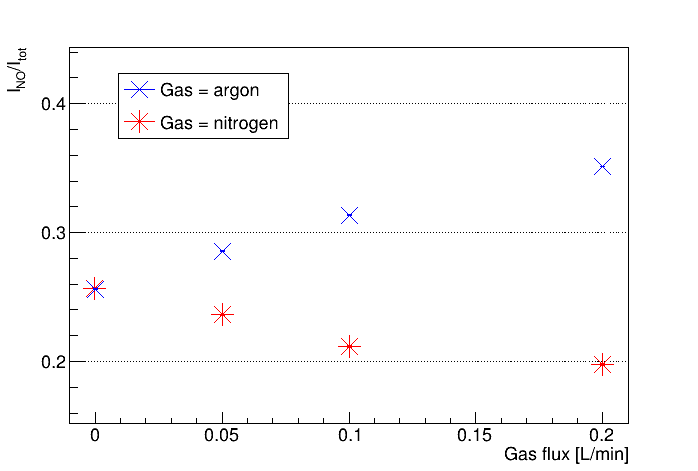
\includegraphics[width=0.45\textwidth]{../Images/Spectroscopy/Irel_NO_flux.png}
 }
 
 \subfloat[Intensità delle righe N2.]{
    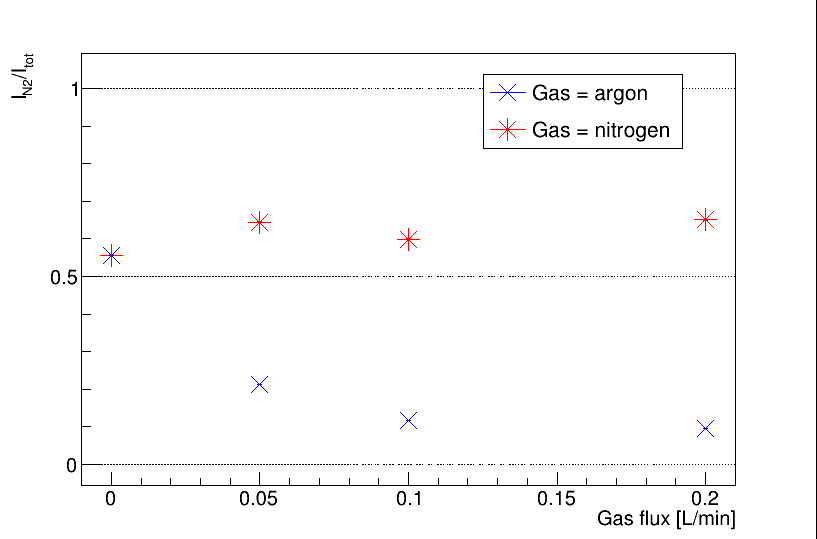
\includegraphics[width=0.45\textwidth]{../Images/Spectroscopy/Irel_N2_flux.png}
 }
 \subfloat[Intensità delle righe di elio.]{
    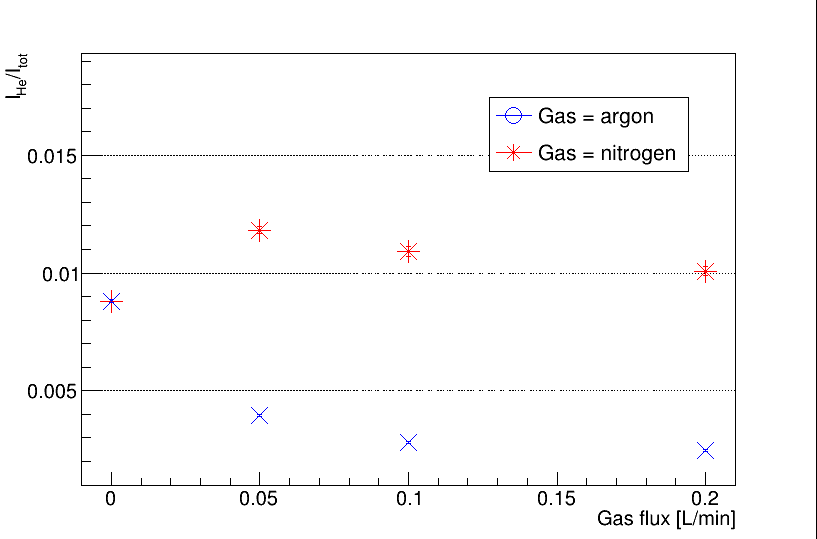
\includegraphics[width=0.45\textwidth]{../Images/Spectroscopy/Irel_He_flux.png}
 }
 
 \subfloat[Intensità delle righe di argon.]{
    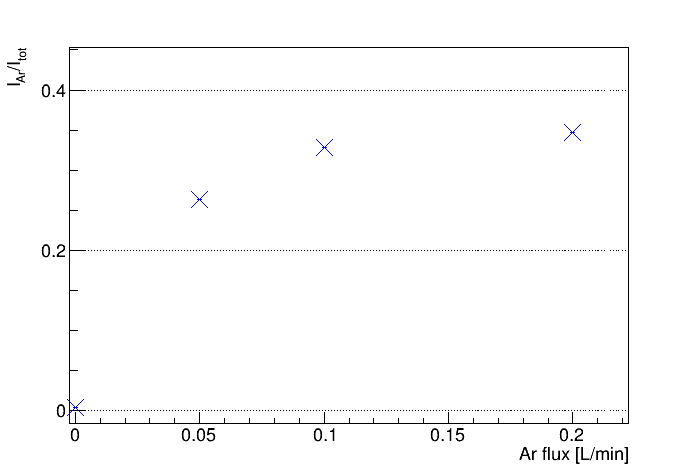
\includegraphics[width=0.45\textwidth]{../Images/Spectroscopy/Irel_Ar_flux.png}
 }
 
 \caption{Intensità delle righe nello spettro al variare del flusso di azoto o argon. La luminosità totale è normalizzata arbitrariamente per i diversi gas, non sono paragonabili i valori per i diversi gas, se ne vuole solo indicare l'andamento. }
 \label{fig:pos}
\end{figure}

\end{document}
